%%%%%%%%%%%%%%%%%%%%%%%%%%%%%%%%%%%%%%%%%%%%%%%%%%%%%%%%%%%%%%%%%%%%%%
% Overleaf (WriteLaTeX) Example: Molecular Chemistry Presentation
%
% Source: http://www.overleaf.com
%
% In these slides we show how Overleaf can be used with standard 
% chemistry packages to easily create professional presentations.
% 
% Feel free to distribute this example, but please keep the referral
% to overleaf.com
% 
%%%%%%%%%%%%%%%%%%%%%%%%%%%%%%%%%%%%%%%%%%%%%%%%%%%%%%%%%%%%%%%%%%%%%%

\documentclass{beamer}

\mode<presentation>
{
  \usetheme{Madrid}       % or try default, Darmstadt, Warsaw, ...
  \usecolortheme{default} % or try albatross, beaver, crane, ...
  \usefonttheme{default}    % or try default, structurebold, ...
  \setbeamertemplate{navigation symbols}{}
  \setbeamertemplate{caption}[numbered]
} 

\usepackage[english]{babel}
\usepackage[utf8x]{inputenc}
\usepackage{chemfig}
\usepackage[version=3]{mhchem}

\usepackage{hyperref}
  \hypersetup{colorlinks=true}
  \hypersetup{urlcolor=blue}
  \hypersetup{linkcolor = .}
\usepackage{xcolor}
\usepackage{siunitx}
  \sisetup{separate-uncertainty = true}
\usepackage{physics}
\usepackage[font=small,labelfont=bf]{caption}
\usepackage{subcaption}
\usepackage[en-GB]{datetime2}
\usepackage{feynmp}
\DeclareGraphicsRule{*}{mps}{*}{}

\usepackage{scalerel}
\newcommand{\mylbrace}[2]{\vspace{#2pt}\hspace{6pt}\scaleleftright[\dimexpr5pt+#1\dimexpr0.06pt]{\lbrace}{\rule[\dimexpr2pt-#1\dimexpr0.5pt]{-4pt}{#1pt}}{.}}
\newcommand{\myrbrace}[2]{\vspace{#2pt}\scaleleftright[\dimexpr5pt+#1\dimexpr0.06pt]{.}{\rule[\dimexpr2pt-#1\dimexpr0.5pt]{-4pt}{#1pt}}{\rbrace}\hspace{6pt}}

% Here's where the presentation starts, with the info for the title slide
\title[$B^\pm\to(K^+K^-\pi^+\pi^-)_DK^\pm$]{\texorpdfstring{$\gamma$}{gamma} analysis update in \texorpdfstring{$B^\pm\to(K^+K^-\pi^+\pi^-)_DK^\pm$}{B to K+K-pi+pi-} decays}
\author{Martin Tat}
\institute{Oxford LHCb}
\date{\today}

\titlegraphic{
\includegraphics[height = 3cm]{lhcb.jpg}\hspace{1cm}~%
              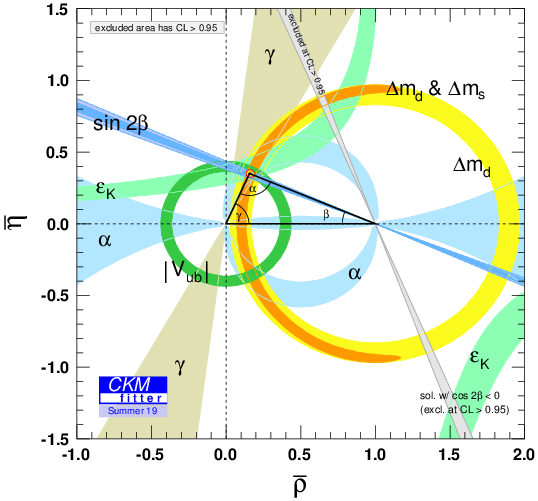
\includegraphics[height = 3cm]{ckmfitter.png}}

\begin{document}

\begin{frame}
  \titlepage
\end{frame}

% These three lines create an automatically generated table of contents.
\begin{frame}{Outline}
  \tableofcontents
\end{frame}

\section{Summary of last time}
\begin{frame}{Summary of last time}
  \begin{itemize}
    \setlength\itemsep{1.2em}
    \item{$B^\pm\to DK^\pm$, $D\to K^+K^-\pi^+\pi^-$, \href{https://arxiv.org/abs/hep-ph/0611272}{arXiv:hep-ph/0611272}}
    \item{Model independent measurement, external strong phase input from BESIII}
    \item{Estimate $2000$ $B$ events from LHCb Run $1$ and $2$}
    \begin{itemize}
      \item{Benchmark: $\sigma(\gamma) = \SI{11}{\degree}$ from model dependent fit}
      \item{LHCb amplitude model in AmpGen, \href{https://arxiv.org/abs/1811.08304}{arXiv:1811.08304}}
    \end{itemize}
    \item{Pull study to test and optimize binning scheme}
    \begin{itemize}
      \item{Simulated $1000$ experiments with $2000$ event each}
      \item{Strong phases from amplitude model using MC integration}
    \end{itemize}
  \end{itemize}
\end{frame}

\section{Binning scheme}
\begin{frame}{Binning scheme}
  \begin{itemize}
    \setlength\itemsep{1.5em}
    \item{Previously: Parameterized 5D phase space and defined binning scheme in terms of $5$ coordinates}
    \item{Better and simpler:}
    \begin{itemize}
      \item{Generate C++ source code for amplitude model using AmpGen}
      \item{Evaluate amplitude directly in analysis}
      \item{Decide bin based on strong phase directly}
    \end{itemize}
  \end{itemize}
  \vspace{1cm}
  \begin{equation*}
    \frac{\mathcal{A}(D^0)}{\mathcal{A}(\bar{D^0})} = r_D\exp(i\delta_D)
  \end{equation*}
\end{frame}



% \section{Binned fit of \texorpdfstring{$D\to K^+K^-\pi^+\pi^-$}{D to K+K-pi+pi-}}
% \begin{frame}{Binned fit of $D\to K^+K^-\pi^+\pi^-$}
%   \vspace{-0.5cm}
%   \begin{align*}
%     \mathcal{A}(B^-\to(K^+K^-\pi^+\pi^-)_DK^-) =& \mathcal{A}_B\mathcal{A}(D^0\to K^+K^-\pi^+\pi^-) \\
%   +& \mathcal{A}_B\mathcal{A}(\bar{D^0}\to K^+K^-\pi^+\pi^-)r_Be^{i(\delta_B - \gamma)}
%   \end{align*}
%   \vspace{-0.5cm}
%   \begin{block}{Event yield in bin $i$}
%     $N^-_i = h_{B^-}\Big(K_i + \big(x_-^2 + y_-^2\big)\bar{K_i} + 2\sqrt{K_i\bar{K_i}}\big(x_-c_i + y_-s_i\big)\Big)$
%     $N^+_i = h_{B^+}\Big(\bar{K_i} + \big(x_+^2 + y_+^2\big)K_i + 2\sqrt{K_i\bar{K_i}}\big(x_+c_i - y_+s_i\big)\Big)$
%   \end{block}
%   \begin{block}{CP-violating observables}
%     $x_\pm = r_B\cos(\delta_B\pm\gamma), \quad y_\pm = r_B\sin(\delta_B\pm\gamma)$
%   \end{block}
%   \begin{itemize}
%     \item{$c_i$, $s_i$: Amplitude-averaged strong phase difference of $D$ decay}
%     \item{Measure $c_i$ and $s_i$ at BES III detector}
%     \item{Can measure $K_i$ and $\bar{K_i}$ at both LHCb and BES III}
%     \item{Need to divide phase space into bins}
%   \end{itemize}
% \end{frame}

% \begin{frame}{Pull studies}
%   \begin{itemize}
%     \item{Pull studies shows that this works}
%     \item{Used an arbitrary and naive binning scheme with $4$ bins}
%     \item{$x_\pm$ pulls show asymmetric tails for $\SI{2e3}{}$ events}
%     \item{$x_\pm$ and $y_\pm$ are all satisfactory for $\SI{2e4}{}$ events}
%   \end{itemize}
%   \begin{block}{Naive binning scheme}
%     Split phase space along the boundaries $E_{K^+} = E_{K_-}$ and $E_{\pi^+} = E_{\pi^-}$ \\
%     Bin $1$: $E_{K^+} > E_{K^-}, \quad E_{\pi^+} > E_{\pi^-}$, \dots
%   \end{block}
%   \begin{block}{$D$ decay hadronic parameters}
%     \begin{equation*}
%       c_i = \frac{\int_i\dd{\Phi}|\mathcal{A}(D^0)||\mathcal{A}(\bar{D^0})|\cos(\delta_D)}{\sqrt{\int_i\dd{\Phi}\abs{\mathcal{A}(D^0)}^2\int_i\dd{\Phi}\abs{\mathcal{A}(D^0)}^2}}, \quad K_i = \frac{\int_i\dd{\Phi}|\mathcal{A}(D^0)|^2}{\sum_j\int_j\dd{\Phi}\abs{\mathcal{A}(D^0)}^2}
%     \end{equation*}
%   \end{block}
% \end{frame}

% \begin{frame}{Pull study with $\SI{2e3}{}$ events}
%   \begin{figure}
%     \centering
%     \vspace{-0.2cm}
%     \begin{subfigure}{0.5\textwidth}
%       \includegraphics[width = 1.0\textwidth]{xplus1K1K.png}
%       \caption{$x_+$ pull}
%     \end{subfigure}%
%     \begin{subfigure}{0.5\textwidth}
%       \includegraphics[width = 1.0\textwidth]{xminus1K1K.png}
%       \caption{$x_-$ pull}
%     \end{subfigure}
%     \begin{subfigure}{0.5\textwidth}
%       \includegraphics[width = 1.0\textwidth]{yplus1K1K.png}
%       \caption{$y_+$ pull}
%     \end{subfigure}%
%     \begin{subfigure}{0.5\textwidth}
%       \includegraphics[width = 1.0\textwidth]{yminus1K1K.png}
%       \caption{$y_-$ pull}
%     \end{subfigure}
%   \end{figure}
% \end{frame}

\end{document}
